\chapter{Analytische Geometrie}

\section{Vektorrechnung}
\begin{flushleft}
Ein Vektor kann als die Verschiebung eines Punktes gesehen werden.
Dabei kann jedoch ein einzelner Vektor auf eine beliebige Menge von Punkten angewandt werden.
Wenn man den Vektor $\vec{a}$ auf den Punkt $P$ anwendet, bekommt man also einen zweiten Punkt $P'$,
dessen Koordinaten um die Werte des Vektors $\vec{a}$ verschoben wurden.

\begin{align}
    \vec{a} &= \begin{pmatrix} 1 \\ 1 \\ 1 \end{pmatrix} \\
    P &= \left(1,2,3\right) \\
    P' &= \left(1+1,2+1,3+1\right) = \left(2,3,4\right)
\end{align}
\end{flushleft}

\begin{center}
\begin{tikzpicture}
\begin{axis}[
    view={35}{15},
    axis lines=center,
    width=15cm,height=15cm,
    xtick={1,2,3,4,5},ytick={1,2,3,4,5},ztick={1,2,3,4,5},
    xmin=0,xmax=5,ymin=0,ymax=5,zmin=0,zmax=5,
    xlabel={$x$},ylabel={$y$},zlabel={$z$}
]

\addplot3 [only marks] coordinates {(1,2,3) (2,3,4)};
\addplot3 [no marks,densely dashed] coordinates {(1,0,0) (1,2,0) (1,2,3) (1,2,0) (0,2,0)};
\addplot3 [no marks,densely dashed] coordinates {(2,0,0) (2,3,0) (2,3,4) (2,3,0) (0,3,0)};

\node [above left] at (axis cs:1,2,3) {$P(1,2,3)$};
\node [above right] at (axis cs:2,3,4) {$P'(2,3,4)$};
\draw [->,thick] (axis cs:1,2,3) to (axis cs:1.97,2.97,3.97);
\node [above left] at (axis cs:1.5,2.5,3.5) {$\vec{a}$};

\end{axis}
\end{tikzpicture}
\end{center}

\subsection{Ortsvektoren}
\begin{flushleft}   
Ortsvektoren verschieben den Ursprung des Koordinatensystems.
Der Ortsvektor $\overrightarrow{OP}$ hat also die gleichen Koordinaten, wie der Punkt $P$,
da $O=(0,0,0)$ ist.

\begin{align}
    O &= (0,0,0) \\
    P &= (1,2,3) \\
    \overrightarrow{OP} &= \begin{pmatrix} 1 \\ 2 \\ 3 \end{pmatrix}
\end{align}
\end{flushleft}

\begin{center}
\begin{tikzpicture}
\begin{axis}[
    view={35}{15},
    axis lines=center,
    width=15cm,height=15cm,
    xtick={1,2,3,4,5},ytick={1,2,3,4,5},ztick={1,2,3,4,5},
    xmin=-2,xmax=5,ymin=-2,ymax=5,zmin=-2,zmax=5,
    xlabel={$x$},ylabel={$y$},zlabel={$z$}
]

\addplot3 [only marks] coordinates {(0,0,0) (1,2,3)};
\addplot3 [no marks,densely dashed] coordinates {(1,0,0) (1,2,0) (1,2,3)};
\addplot3 [no marks,densely dashed] coordinates {(0,2,0) (1,2,0)};

\node [above right] at (axis cs:1,2,3) {$P(1,2,3)$};
\node [left] at (axis cs:0,0,0) {$O(0,0,0)$};
\draw [->,thick] (axis cs:0,0,0) to (axis cs:0.95,1.95,2.95);
\node [below] at (axis cs:0.3,1.3,2.3) {$\overrightarrow{OP}$};

\end{axis}
\end{tikzpicture}
\end{center}

\subsection{Addition}
\begin{flushleft}
Die Addition von Vektoren ist sehr simpel.
Wenn $\vec{a}$ und $\vec{b}$ addiert werden sollen, werden alle Einträge von $\vec{b}$
zu den Einträgen von $\vec{a}$ addiert.
\begin{align}
    \vec{a} &= \begin{pmatrix} 1 \\ 1 \\ 1 \end{pmatrix} \\
    \vec{b} &= \begin{pmatrix} 2 \\ 3 \\ 4 \end{pmatrix} \\
    \vec{a}+\vec{b} &= \begin{pmatrix} 1+2 \\ 1+3 \\ 1+4 \end{pmatrix} \\
    \vec{a}+\vec{b} &= \begin{pmatrix} 3 \\ 4 \\ 5 \end{pmatrix}
\end{align}
\end{flushleft}

\begin{center}
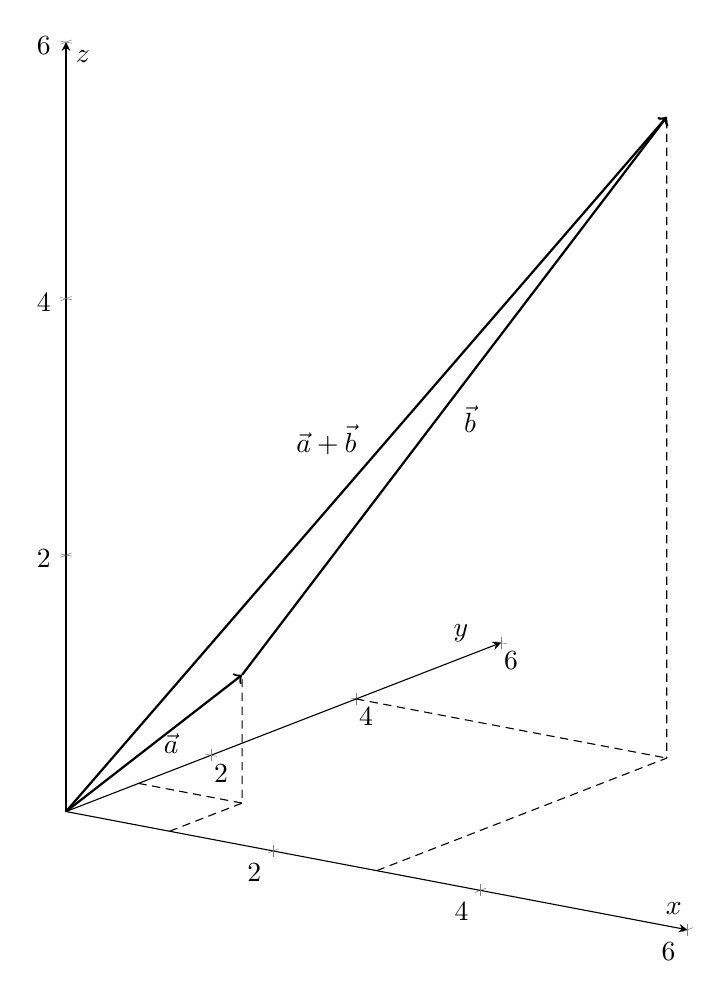
\begin{tikzpicture}
\begin{axis}[
    view={35}{15},
    axis lines=center,
    width=15cm,height=15cm,
    xtick={2,4,6},ytick={2,4,6},ztick={2,4,6},
    xmin=0,xmax=6,ymin=0,ymax=6,zmin=0,zmax=6,
    xlabel={$x$},ylabel={$y$},zlabel={$z$}
]

\addplot3 [no marks,densely dashed] coordinates {(1,0,0) (1,1,0) (1,1,1)};
\addplot3 [no marks,densely dashed] coordinates {(0,1,0) (1,1,0)};

\addplot3 [no marks,densely dashed] coordinates {(3,0,0) (3,4,0) (3,4,5)};
\addplot3 [no marks,densely dashed] coordinates {(0,4,0) (3,4,0)};

\draw [->,thick] (axis cs:0,0,0) to (axis cs:1,1,1);
\node [right] at (axis cs:0.5,0.5,0.5) {$\vec{a}$};

\draw [->,thick] (axis cs:1,1,1) to (axis cs:3,4,5);
\node [below right] at (axis cs:2,2.5,3) {$\vec{b}$};

\draw [->,thick] (axis cs:0,0,0) to (axis cs:3,4,5);
\node [above left] at (axis cs:1.5,2,2.5) {$\vec{a}+\vec{b}$};

\end{axis}
\end{tikzpicture}
\end{center}

\subsection{Multiplikation}
\begin{flushleft}    
Ein Vektor kann mit einer Zahl $r \in \mathbb{R}$ multipliziert werden.
Ähnlich wie bei der Addition werden hier alle Einträge eines Vektors mit $r$ multipliziert.

\begin{align}
    \vec{a} &= \begin{pmatrix} 1 \\ 2 \\ 3 \end{pmatrix} \\
    r &= 2 \\
    2\vec{a} &= \begin{pmatrix} 2 \cdot 1 \\ 2 \cdot 2 \\ 2 \cdot 3 \end{pmatrix} = \begin{pmatrix} 2 \\ 4 \\ 6 \end{pmatrix}
\end{align}
\end{flushleft}

\begin{center}
\begin{tikzpicture}
\begin{axis}[
    view={35}{15},
    axis lines=center,
    width=15cm,height=15cm,
    xtick={2,4,6},ytick={2,4,6},ztick={2,4,6},
    xmin=0,xmax=6,ymin=0,ymax=6,zmin=0,zmax=6,
    xlabel={$x$},ylabel={$y$},zlabel={$z$}
]

\addplot3 [no marks,densely dashed] coordinates {(1,0,0) (1,2,0) (1,2,3)};
\addplot3 [no marks,densely dashed] coordinates {(0,2,0) (1,2,0)};

\addplot3 [no marks,densely dashed] coordinates {(2,0,0) (2,4,0) (2,4,6)};
\addplot3 [no marks,densely dashed] coordinates {(0,4,0) (2,4,0)};

\draw [->,thick,red] (axis cs:1,2,3) to (axis cs:2,4,6);
\node [below right] at (axis cs:1.5,3,4.5) {$2\vec{a}$};

\draw [->,thick,blue] (axis cs:0,0,0) to (axis cs:1,2,3);
\node [right] at (axis cs:0.5,1,1.5) {$\vec{a}$};

\end{axis}
\end{tikzpicture}
\end{center}

\begin{flushleft}
Der Vektor $\vec{a}$ wird hier um $r$ verlängert.
In diesem Beispiel wird $\vec{a}$ also doppelt so lang, da $r=2$ ist.
Falls $\left| r \right| < 1$ ist, wird der Vektor $\vec{a}$ also verkürzt.

\begin{align}
    \vec{a} &= \begin{pmatrix} 1 \\ 2 \\ 3 \end{pmatrix} \\
    r &= \frac{1}{2} \\
    \frac{1}{2} \vec{a} &= \begin{pmatrix} \frac{1}{2} \cdot 1 \\ \frac{1}{2} \cdot 2 \\ \frac{1}{2} \cdot 3 \end{pmatrix} = \begin{pmatrix} \frac{1}{2} \\ 1 \\ \frac{3}{2} \end{pmatrix}
\end{align}
\end{flushleft}

\begin{center}
\begin{tikzpicture}
\begin{axis}[
    view={35}{15},
    axis lines=center,
    width=15cm,height=15cm,
    xtick={2,4,6},ytick={2,4,6},ztick={2,4,6},
    xmin=0,xmax=6,ymin=0,ymax=6,zmin=0,zmax=6,
    xlabel={$x$},ylabel={$y$},zlabel={$z$}
]

\addplot3 [no marks,densely dashed] coordinates {(1,0,0) (1,2,0) (1,2,3)};
\addplot3 [no marks,densely dashed] coordinates {(0,2,0) (1,2,0)};

\addplot3 [no marks,densely dashed] coordinates {(0.5,0,0) (0.5,1,0) (0.5,1,1.5)};
\addplot3 [no marks,densely dashed] coordinates {(0,1,0) (0.5,1,0)};

\draw [->,thick,blue] (axis cs:0,0,0) to (axis cs:0.5,1,1.5);
\node [right] at (axis cs:0.25,0.5,0.75) {$\frac{1}{2}\vec{a}$};

\draw [->,thick,red] (axis cs:0.5,1,1.5) to (axis cs:1,2,3);
\node [below right] at (axis cs:0.75,1.5,2.25) {$\vec{a}$};

\end{axis}
\end{tikzpicture}
\end{center}

\begin{flushleft}
Nach dem selben Prinzip wird die Richtung von $\vec{a}$ getauscht, wenn $r < 0$ ist.
\end{flushleft}

\begin{center}
\begin{tikzpicture}
\begin{axis}[
    view={35}{15},
    axis lines=center,
    width=15cm,height=15cm,
    xtick={1,2,3,4},ytick={1,2,3,4},ztick={1,2,3,4},
    xmin=0,xmax=4,ymin=0,ymax=4,zmin=0,zmax=4,
    xlabel={$x$},ylabel={$y$},zlabel={$z$}
]

\addplot3 [no marks,densely dashed] coordinates {(1,0,0) (1,2,0) (1,2,3)};
\addplot3 [no marks,densely dashed] coordinates {(0,2,0) (1,2,0)};

\addplot3 [no marks,densely dashed] coordinates {(0.5,0,0) (0.5,1,0) (0.5,1,1.5)};
\addplot3 [no marks,densely dashed] coordinates {(0,1,0) (0.5,1,0)};

\draw [->,thick,red] (axis cs:0,0,0) to (axis cs:1,2,3);
\node [below right,red] at (axis cs:0.25,0.5,0.75) {$\vec{a}$};

\draw [->,thick,blue] (axis cs:1,2,3) to (axis cs:0.5,1,1.5);
\node [right,blue] at (axis cs:0.75,1.5,2.25) {$\frac{-1}{2}\vec{a}$};

\end{axis}
\end{tikzpicture}
\end{center}

\begin{flushleft}
Wenn $\vec{a}$ mit $-1$ multipliziert wird, entsteht sein Gegenvektor $-\vec{a}$,
der die gleiche länge wie $\vec{a}$ hat aber in die andere Richtung zeigt.
\end{flushleft}

\begin{center}
\begin{tikzpicture}
\begin{axis}[
    view={35}{15},
    axis lines=center,
    width=15cm,height=15cm,
    xtick={1,2,3,4},ytick={1,2,3,4},ztick={1,2,3,4},
    xmin=0,xmax=4,ymin=0,ymax=4,zmin=0,zmax=4,
    xlabel={$x$},ylabel={$y$},zlabel={$z$}
]

\addplot3 [no marks,densely dashed] coordinates {(1,0,0) (1,2,0) (1,2,3)};
\addplot3 [no marks,densely dashed] coordinates {(0,2,0) (1,2,0)};

%\addplot3 [no marks,densely dashed] coordinates {(0.5,0,0) (0.5,1,0) (0.5,1,1.5)};
%\addplot3 [no marks,densely dashed] coordinates {(0,1,0) (0.5,1,0)};

\draw [->,thick,red] (axis cs:0,0,0) to (axis cs:1,2,3);
\node [below right,red] at (axis cs:0.5,1,1.5) {$\vec{a}$};

\draw [->,thick,blue] (axis cs:1,2,3) to (axis cs:0,0,0);
\node [above left,blue] at (axis cs:0.5,1,1.5) {$-\vec{a}$};

\end{axis}
\end{tikzpicture}
\end{center}
